\documentclass[a4paper,12pt]{article}

\setlength{\parindent}{1.25cm} % Установка абзацного отступа в 1.25 см

% Пакеты

% Пакеты для поддержки кириллицы
\usepackage[utf8]{inputenc}    % Кодировка UTF-8
\usepackage[T2A]{fontenc}      % Поддержка кириллицы
\usepackage[english,russian]{babel} % Русский и английский языки
\usepackage{mathptmx}          % Используем шрифт Times New Roman вместо Computer Modern

\usepackage{amsmath,amsfonts,amssymb} % Математические символы
\usepackage{graphicx}          % Для вставки изображений
\usepackage{geometry}          % Настройка полей
\usepackage{float}             % Фиксация местоположения таблиц и рисунков
\usepackage{hyperref}          % Ссылки
\usepackage{titlesec}          % Для оформления заголовков разделов
\usepackage{xcolor}			  % Цвета

\usepackage{longtable} % Для длинных таблиц, если нужно
\usepackage{array}     % Для улучшенного контроля над таблицами
\usepackage{makecell} % Пакет для работы с многострочными ячейками

\usepackage{hyperref} % Пакет для гиперссылок (в источниках)

% Настройка полей
\geometry{
    left=30mm,
    right=15mm,
    top=20mm,
    bottom=20mm
}

% Настройка стиля заголовков
\titleformat{\section}{\large\bfseries}{\thesection.}{1em}{}
\titleformat{\subsection}{\normalsize\bfseries}{\thesubsection.}{1em}{}

% Для кода
\usepackage{listings}
% Настройка стиля для кода
\lstset{
    language=Python,            % Язык кода
    basicstyle=\ttfamily\footnotesize,  % Базовый стиль текста и размер шрифта
    backgroundcolor=\color{gray!10},    % Цвет фона
    frame=single,              % Рамка вокруг листинга
    breaklines=true,           % Переносить строки
    captionpos=b,              % Позиция заголовка (caption) снизу
    tabsize=4,                 % Размер табуляции
    commentstyle=\color{gray}, % Стиль комментариев
    keywordstyle=\color{blue}, % Стиль ключевых слов
    stringstyle=\color{red},   % Стиль строк
    showstringspaces=false,    % Не отображать пробелы в строках
    numberstyle=\tiny\color{gray} % Стиль номеров строк
}


\begin{document}

% Титульный лист
\begin{titlepage}
    \centering
    {\bfseries Министерство науки и высшего образования Российской Федерации}\\
    {\bfseries Московский государственный технический университет им. Н. Э. Баумана}\\
    Кафедра ИУ7 «Программное обеспечение ЭВМ и информационные технологии» \\
    \vfill
    % Вставка герба МГТУ им. Баумана
    
\includegraphics[width=0.5\textwidth]{gerb.png} % путь к изображению и размер
    \vfill
    % Увеличенный шрифт для надписи "ОТЧЁТ"
    {\fontsize{17}{22}\selectfont \textbf{\underline{ОТЧЁТ}}}\\[0.5cm]
    {\fontsize{14.4}{20}\selectfont по лабораторной работе №1\\
    по курсу «Анализ алгоритмов»\\
    Тема: «Расстояние Левенштейна и Дамерау-Левенштейна»}\\
    \vfill
    Выполнила: студентка группы ИУ7-55Б Талышева О.Н.\\
    Преподаватель: Строганов Ю.В.
    \vfill
    Москва, 2024
\end{titlepage}

% Оглавление
\tableofcontents
\newpage

% Введение
\section*{Введение}
\subsection*{Цель}
Цель лабораторной работы: исследовать алгоритмы вычисления расстояния Левенштейна и Дамерау-Левенштейна в матричной, рекурсивно-матричной и рекурсивной реализациях.
\subsection*{Задачи}
Для достижения этой цели были поставлены следующие задачи:\\
\begin{itemize}
\item изучить алгоритм вычисления расстояния Левенштейна
\item изучить алгоритм вычисления расстояния Дамерау-Левенштейна
\item применить метод динамического программирования для матричных реализаций алгоритмов
\item сравнить матричную, рекурсивно-матричную и рекурсивную реализации алгоритмов
\item сравнить алгоритмы вычисления расстояния Левенштейна и Дамерау-Левенштейна
\end{itemize}
\newpage

% Основная часть
\section{Аналитическая часть}
\subsection{Редакционное расстояние между двумя строками}
Часто требуется измерить различие или расстояние между двумя строками (например, в эволюционных, структуральных или функциональных исследованиях биологических строк, в хранении текстовых баз данных, в методах проверки правописания). Есть несколько способов формализации понятия расстояния между строками. Одна общая и простая, формализация называется редакционным расстоянием; она основана на преобразовании (или редактировании) одной строки в другую серией операций редактирования, выполняемых над отдельными символами. Разрешенные операции редактирования — это вставка (I - insertion) символа в первую строку, удаление (D - deletion) символа из первой строки и подстановка или замена (substitution или, лучше, R - replace) символа из первой строки символом из второй строки. Обозначим M — “не-операцию“ над правильной буквой (от match).\\
Строка над алфавитом 1, D, R , М, которая описывает преобразование одной строки в другую, называется редакционным предписанием (предписанием) этих двух строк.\\
Редакционное расстояние между двумя строками определяется как минимальное число редакционных операций — вставок, удалений и подстановок, необходимое для преобразования первой строки во вторую.\\
Подчеркнем, что совпадения операциями не являются и не засчитываются.
Редакционное расстояние иногда называют расстоянием Левенштейна по статье В. Левенштейна, где оно рассматривалось, вероятно, впервые.
\subsection{Выравнивание строк}
Редакционное предписание — это способ представления конкретного преобразования одной строки в другую. Альтернативный (и часто предпочтительный) способ заключается в показе явного выравнивания (alignment) этих двух строк.\\
(Глобальное) выравнивание двух строк, Sl и S2, получается вставкой пробелов в строки S1 и S2 (возможно, на их концах) и размещением двух получившихся строк друг над другом так, чтобы каждый символ или пробел одной строки оказался напротив одного символа или пробела другой строки.\\
Термин «глобальный» подчёркивает, что обе строки участвуют в выравнивании полностью.\cite{gasfild}
\subsection{Расстояние Левенштейна}
Расстояние Левенштейна, или редакционное расстояние, — метрика cходства между двумя строковыми последовательностями. Чем больше расстояние, тем более различны строки. По сути, это минимальное число односимвольных преобразований (удаления, вставки или замены), необходимых, чтобы превратить одну последовательность в другую.\\
Цены операций могут зависеть от вида операции (вставка, удаление, замена) и/или от участвующих в ней символов, отражая разную вероятность мутаций в биологии, разную вероятность разных ошибок при вводе текста и т. д. В общем случае:\\
\begin{itemize}
\item D(a, b) — цена замены символа a на символ b
\item D($\lambda$, b) — цена вставки символа b
\item D(a, $\lambda$) — цена удаления символа a
\end{itemize}
Необходимо найти последовательность замен, минимизирующую суммарную цену. Расстояние Левенштейна является частным случаем этой задачи при ценах:\\
\begin{itemize}
\item D(a, а) = 0
\item D(a, b) = 1, при a $\neq$ b
\item D($\lambda$, b) = 1
\item D(a, $\lambda$) = 1
\end{itemize}
Как частный случай, так и задачу для произвольных D, решает алгоритм Вагнера — Фишера, приведённый ниже. Здесь и ниже считается, что все D неотрицательны, и действует неравенство треугольника: замена двух последовательных операций одной не увеличит общую цену (например, замена символа x на y, а потом y на z не лучше, чем сразу x на z).\\
Например, D(’hello’, ‘hallo’) = 1, так как потребуется провести одну замену ‘e’ на ‘a’.\\
Алгоритм реализуется по следующей формуле:\\
\[
d(S_1, S_2) = D(M, N), \text{где}\\
D(i, j) = 
\begin{cases}
0,  & \text{i = 0, j = 0} \\
i,  & \text{i > 0, j = 0} \\
j,  & \text{i = 0, j > 0} \\
\min
\begin{cases}
D(i-1, j) + 1 & \text{(удаление)} \\
D(i, j-1) + 1 & \text{(вставка)} \\
D(i-1, j-1) + 1_{\text{если}\,a_i \neq b_j} & \text{(замена)}
\end{cases}  & \text{i > 0, j > 0}
\end{cases}
\]\\
Таким образом, требуется вычислить матрицу расстояний размерностью $len(str_1) * len(str_2)$, следовательно, объем требуемой памяти растет как $O(len(str_1) * len(str_2))$. Иными словами, для двух мегабайтных строк потребуются гигабайты памяти. Фактически в кэше будет хранится почти все матрица редактирований, а она не нужна целиком. Искомая цель – правый нижний элемент.\\[0.1cm]
\begin{figure} [H] % Принудительное размещение изображения
	\centering    
    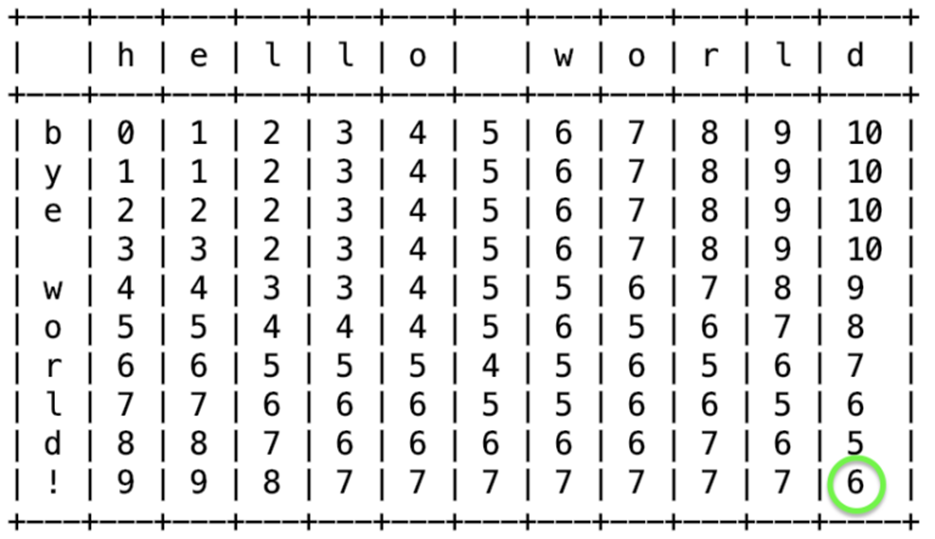
\includegraphics[width=0.8\textwidth]{exampleLeven.png} % путь к изображению и размер
    \caption{Пример нахождения расстояния Левенштейна}
\end{figure}
Для его поиска можно обойтись лишь парой рядов: текущим и предыдущим. А остальные ряды не хранить в памяти. Так будет достигнут конец таблицы, и нижний правый угол и будет искомым значением.\\
Чтобы использовать еще меньше памяти, можно поменять местами строки, чтобы длина рядов была минимальна. Это существенно экономит память, если одна из строк длинная, а другая короткая.
\subsection{Расстояние Дамерау-Левенштейна}
Если к списку разрешённых операций добавить транспозицию (два соседних символа меняются местами), получается расстояние Дамерау — Левенштейна. Для неё также существует алгоритм, требующий O(len(str1) * len(str2)) операций. Дамерау показал, что 80\% ошибок при наборе текста человеком являются транспозициями. Кроме того, расстояние Дамерау-Левенштейна используется и в биоинформатике.\\
Цена операции транспозиция также равна 1. При работе алгоритма Левенштейна эта операция реализовалась бы двумя заменами и стоила бы 2. Таким образом, расстояние Дамерау-Левенштейна в некоторых случаях даёт меньший результат, чем расстояние Левенштейна.\\
В алгоритм добавляется следующая формула:\\

\[
\begin{cases}
i > 1 \\
j > 1 \\
\text{str}_1[i-1] = \text{str}_2[j] \\
\text{str}_1[i] = \text{str}_2[j-1]
\end{cases}
\]
\newpage

% Рисуночки
\section{Конструкторская часть}
\subsection*{Схемы алгоритмов}
На основании теоретических измышлений были разработаны алгоритмы, вычисляющие расстояние Левенштейна и Дамерау-Левенштейна тремя способами:\\
\begin{figure}[H]
    \centering
    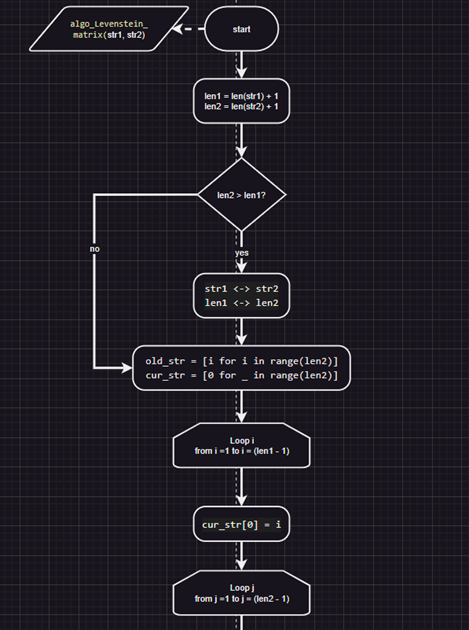
\includegraphics[width=0.7\textwidth]{block_1_1_1.png}
    \caption{Блоксхема алгоритма Левенштейна (матричная реализация)}
\end{figure}
\begin{figure}[H]
    \centering
    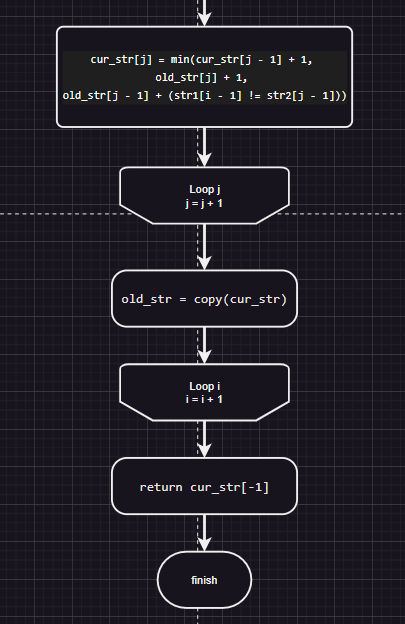
\includegraphics[width=0.7\textwidth]{block_1_1_2.png}
    \caption{Блоксхема алгоритма Левенштейна (матричная реализация) (продолжение)}
\end{figure}
\begin{figure}[H]
    \centering
    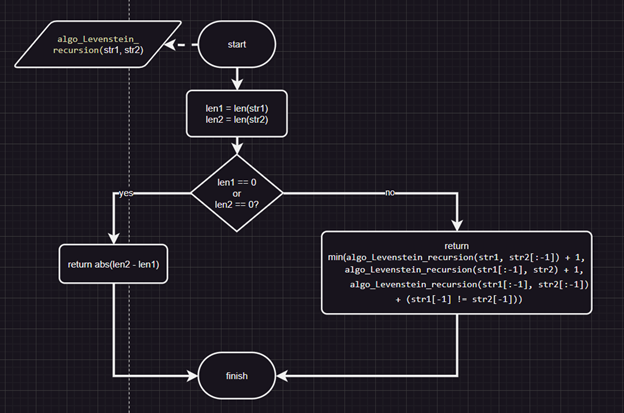
\includegraphics[width=1\textwidth]{block_1_2.png}
    \caption{Блоксхема алгоритма Левенштейна (рекурсивная реализация)}
\end{figure}
\begin{figure}[H]
    \centering
    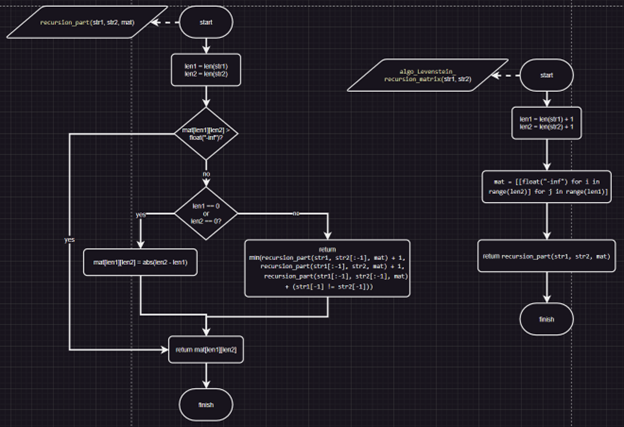
\includegraphics[width=1\textwidth]{block_1_3.png}
    \caption{Блоксхема алгоритма Левенштейна (рекурсивно-матричная реализация)}
\end{figure}
\begin{figure}[H]
    \centering
    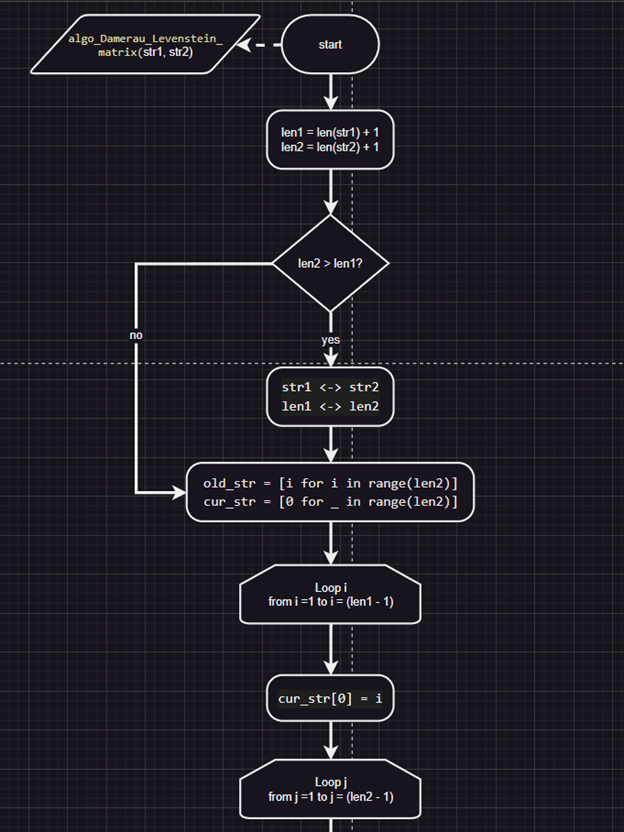
\includegraphics[width=0.8\textwidth]{block_2_1_1.png}
    \caption{Блоксхема алгоритма Дамерау-Левенштейна (матричная реализация)}
\end{figure}
\begin{figure}[H]
    \centering
    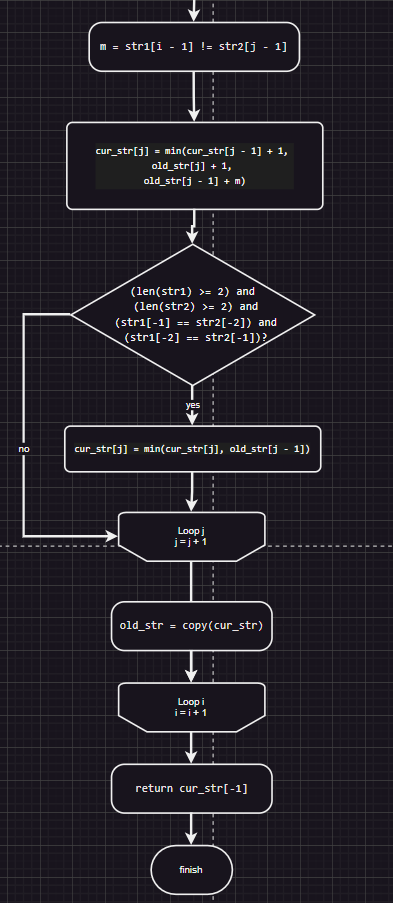
\includegraphics[width=0.7\textwidth]{block_2_1_2.png}
    \caption{Блоксхема алгоритма Дамерау-Левенштейна (матричная реализация) (продолжение)}
\end{figure}
\begin{figure}[H]
    \centering
    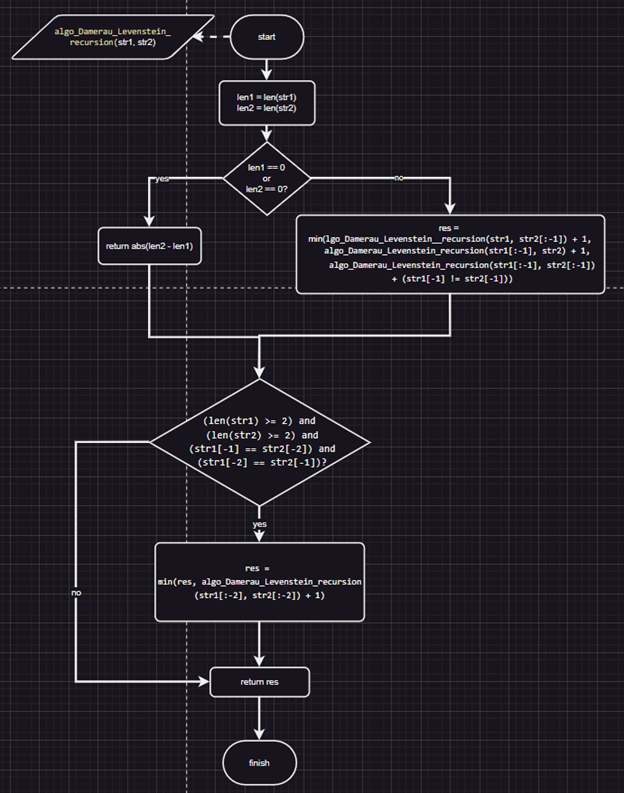
\includegraphics[width=1\textwidth]{block_2_2.png}
    \caption{Блоксхема алгоритма Дамерау-Левенштейна (рекурсивная реализация)}
\end{figure}
\begin{figure}[H]
    \centering
    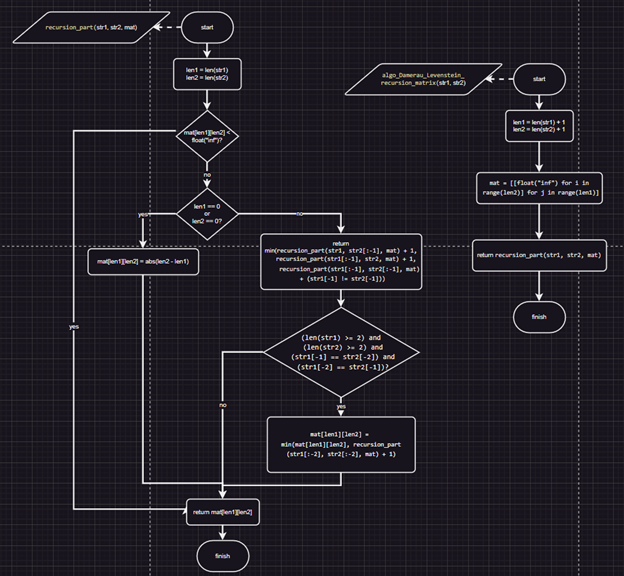
\includegraphics[width=1\textwidth]{block_2_3.png}
    \caption{Блоксхема алгоритма Дамерау-Левенштейна (рекурсивно-матричная реализация)}
\end{figure}
\newpage

\section{Технологическая часть}
\subsection{Требования к программному обеспечению}
На вход программе подаются 2 строки из символов, которые входят в таблицу Юникода (UTF-8).\par
На выход программа выдаёт число – расстояние между строками, вычисленное алгоритмом Левенштейна или Дамерау-Левенштейна матричной или рекурсивной реализацией. Для матричных реализаций также выводится матрица расстояний. Также в зависимости от выбранного пункта меню программа замеряет время работы алгоритмов и рисует получившиеся графики.
\subsection{Средства реализации}
Python быстро работает с алгоритмами Левенштейна и Дамерау-Левенштейна благодаря эффективной обработке строк и богатой библиотеке, что делает его идеальным для задач текстового сравнения и редактирования. Поэтому программа была реализована на языке Python, для замеров времени была использована функция \texttt{process\_time()} из библиотеки \texttt{time}, вычисляющая процессорное время\cite{process_time}.
\subsection{Реализации алгоритмов}
\begin{lstlisting}[caption=реализация матричного алгоритма Левенштейна]
def algo_Levenstein_matrix(str1: str, str2: str) -> int:
    len1, len2 = len(str1) + 1, len(str2) + 1
    if len2 > len1:
        str1, str2 = str2, str1
        len1, len2 = len2, len1
    old_str = [i for i in range(len2)]
    cur_str = [0 for _ in range(len2)]
    for i in range(1, len1):
        cur_str[0] = i
        for j in range(1, len2):
            cur_str[j] = min(cur_str[j - 1] + 1,
                            old_str[j] + 1,
                            old_str[j - 1] + (str1[i - 1] != str2[j - 1]))
        old_str = cur_str.copy()
    return cur_str[-1]
\end{lstlisting}
\begin{lstlisting}[caption=реализация рекурсивного алгоритма Левенштейна]
def algo_Levenstein_recursion(str1: str, str2: str) -> int:
    len1, len2 = len(str1), len(str2)
    if len1 * len2 == 0:
        return abs(len2 - len1)
    return min(algo_Levenstein_recursion(str1, str2[:-1]) + 1,
                algo_Levenstein_recursion(str1[:-1], str2) + 1,
                algo_Levenstein_recursion(str1[:-1], str2[:-1]) + (str1[-1] != str2[-1]))
\end{lstlisting}
\begin{lstlisting}[caption=реализация рекурсивно-матричного алгоритма Левенштейна]
def algo_Levenstein_recursion_matrix(str1: str, str2: str) -> int:
    len1, len2 = len(str1) + 1, len(str2) + 1
    mat = [[float("-inf") for i in range(len2)] for j in range(len1)]
    # the recursive part itself
    def recursion_part(str1: str, str2: str, mat: List[float] = []) -> int:
        len1, len2 = len(str1), len(str2)
        if mat[len1][len2] > float("-inf"):
            pass
        elif len1 * len2 == 0:
            mat[len1][len2] = abs(len2 - len1)
        else:
            mat[len1][len2] = min(recursion_part(str1, str2[:-1], mat) + 1,
                    recursion_part(str1[:-1], str2, mat) + 1,
                    recursion_part(str1[:-1], str2[:-1], mat) + (str1[-1] != str2[-1]))
        return mat[len1][len2]
    return recursion_part(str1, str2, mat)
\end{lstlisting}
\begin{lstlisting}[caption=реализация матричного алгоритма Дамерау-Левенштейна]
def algo_Damerau_Levenstein_matrix(str1: str, str2: str) -> int:
    len1, len2 = len(str1) + 1, len(str2) + 1
    if len2 > len1:
        str1, str2 = str2, str1
        len1, len2 = len2, len1
    old_str = [i for i in range(len2)]
    cur_str = [0 for _ in range(len2)]
    for i in range(1, len1):
        cur_str[0] = i
        for j in range(1, len2):
            m = str1[i - 1] != str2[j - 1]
            cur_str[j] = min(cur_str[j - 1] + 1,
                            old_str[j] + 1,
                            old_str[j - 1] + m)
            if (i > 1) and (j > 1) and m and (str1[i - 2] == str2[j - 1]) and (str1[i - 1] == str2[j - 2]):
                cur_str[j] = min(cur_str[j], old_str[j - 1])
        old_str = cur_str.copy()
    return cur_str[-1]
\end{lstlisting}
\begin{lstlisting}[caption=реализация рекурсивного алгоритма Дамерау-Левенштейна]
def algo_Damerau_Levenstein_recursion(str1: str, str2: str) -> int:
    len1, len2 = len(str1), len(str2)
    if len1 * len2 == 0:
        return abs(len2 - len1)
    res = min(algo_Damerau_Levenstein_recursion(str1, str2[:-1]) + 1,
                algo_Damerau_Levenstein_recursion(str1[:-1], str2) + 1,
                algo_Damerau_Levenstein_recursion(str1[:-1], str2[:-1]) + (str1[-1] != str2[-1]))
    if ((len(str1) >= 2) and (len(str2) >= 2) and (str1[-1] == str2[-2]) and (str1[-2] == str2[-1])):
        res = min(res, algo_Damerau_Levenstein_recursion(str1[:-2], str2[:-2]) + 1)
    return res
\end{lstlisting}
\begin{lstlisting}[caption=реализация рекурсивно-матричного алгоритма Дамерау-Левенштейна]
def algo_Damerau_Levenstein_recursion_matrix(str1: str, str2: str) -> int:
    len1, len2 = len(str1) + 1, len(str2) + 1
    mat = [[float("inf") for i in range(len2)] for j in range(len1)]
    # the recursive part itself
    def recursion_part(str1: str, str2: str, mat: List[float] = []) -> int:
        len1, len2 = len(str1), len(str2)
        if mat[len1][len2] < float("inf"):
            pass
        elif len1 * len2 == 0:
            mat[len1][len2] = abs(len2 - len1)
        else:
            mat[len1][len2] = min(recursion_part(str1, str2[:-1], mat) + 1,
                    recursion_part(str1[:-1], str2, mat) + 1,
                    recursion_part(str1[:-1], str2[:-1], mat) + (str1[-1] != str2[-1]))
            if ((len(str1) >= 2) and (len(str2) >= 2) and (str1[-1] == str2[-2]) and (str1[-2] == str2[-1])):
                mat[len1][len2] = min(mat[len1][len2], recursion_part(str1[:-2], str2[:-2], mat) + 1)
        return mat[len1][len2]
    return recursion_part(str1, str2, mat)
\end{lstlisting}
\subsection{Тесты}
\begin{table}[H]
    \centering
    \begin{tabular}{|c|c|c|c|c|c|}
        \hline
        \textbf{Строка 1} & \textbf{Строка 2} & \textbf{Ожидание} & \textbf{матричный} & \textbf{рекурсивный} & \makecell{\textbf{рекурсивно-}\\\textbf{матричный}} \\
        \hline
        $\lambda$ & $\lambda$ & 0 & 0 & 0 & 0 \\
        a  & a  & 0 & 0 & 0 & 0 \\
        abc & abc & 0 & 0 & 0 & 0 \\
        $\lambda$  & a  & 1 & 1 & 1 & 1 \\
        a  & $\lambda$  & 1 & 1 & 1 & 1 \\
        a  & b  & 1 & 1 & 1 & 1 \\
        abc & abs & 1 & 1 & 1 & 1 \\
        odc & abc & 2 & 2 & 2 & 2 \\
        ods & abc & 3 & 3 & 3 & 3 \\
        abcs & abc & 1 & 1 & 1 & 1 \\
        bc & abc & 1 & 1 & 1 & 1 \\
        bac & abc & 2 & 2 & 2 & 2 \\
        \hline
    \end{tabular}
    \caption{Таблица тестов для алгоритмов Левенштейна}
\end{table}
\begin{table}[H]
    \centering
    \begin{tabular}{|c|c|c|c|c|c|}
        \hline
        \textbf{Строка 1} & \textbf{Строка 2} & \textbf{Ожидание} & \textbf{матричный} & \textbf{рекурсивный} & \makecell{\textbf{рекурсивно-}\\\textbf{матричный}} \\
        \hline
        $\lambda$ & $\lambda$ & 0 & 0 & 0 & 0 \\
        a  & a  & 0 & 0 & 0 & 0 \\
        abc & abc & 0 & 0 & 0 & 0 \\
        $\lambda$  & a  & 1 & 1 & 1 & 1 \\
        a  & $\lambda$  & 1 & 1 & 1 & 1 \\
        a  & b  & 1 & 1 & 1 & 1 \\
        abc & abs & 1 & 1 & 1 & 1 \\
        odc & abc & 2 & 2 & 2 & 2 \\
        ods & abc & 3 & 3 & 3 & 3 \\
        abcs & abc & 1 & 1 & 1 & 1 \\
        bc & abc & 1 & 1 & 1 & 1 \\
        bac & abc & 1 & 1 & 1 & 1 \\
        \hline
    \end{tabular}
    \caption{Таблица тестов для алгоритмов Дамерау-Левенштейна}
\end{table}
В ходе проведённого тестирования (с помощью pytest) ошибок в алгоритмах не выявлено:\\[0.1cm]
\begin{figure}[H]  % Принудительное размещение изображения
    \centering
    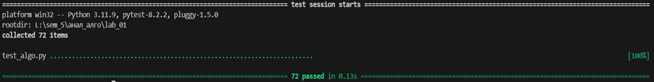
\includegraphics[width=1\textwidth]{pytest_result.png}
    \caption{Результаты тестов с использованием pytest}
\end{figure}
\newpage

% Исследовательская часть
\section{Исследовательская часть}
Для сравнения времени реализаций алгоритмов Левенштейна и Дамерау-Левенштейна в их матричных и рекурсивных реализациях программа была запущена на рандомно сгенерированных строках длинами от 1 до 9 с шагом 2 по 50 замеров каждая строка, среднее значение было вынесено в таблицу и для наглядности изображено на графике:\par
\begin{figure}[H]
    \centering
    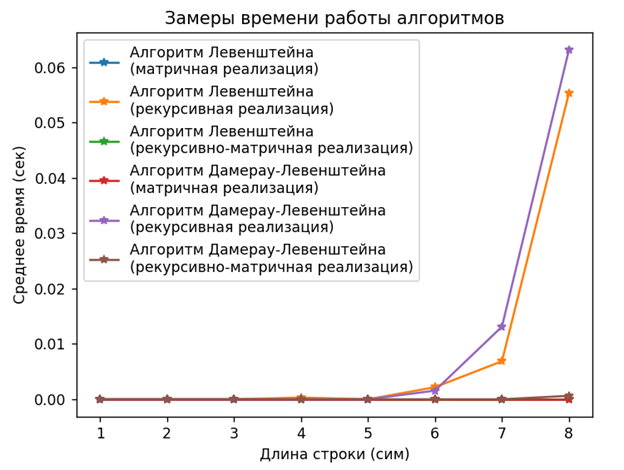
\includegraphics[width=1\textwidth]{graph_all.png}
    \caption{График времени работы всех алгоритмов в зависимости от длин строк}
\end{figure}
\begin{figure}[H]
    \centering
    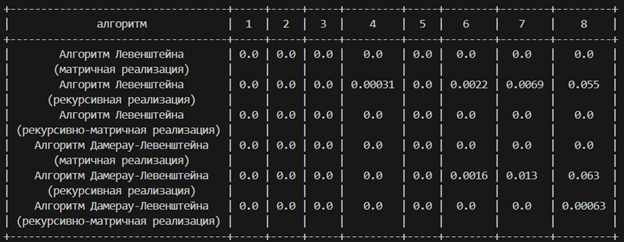
\includegraphics[width=1\textwidth]{table_all.png}
    \caption{Таблица времени работы всех алгоритмов в зависимости от длин строк}
\end{figure}
\subsection{Сравнение работы матричной, рекурсивной и рекурсивно-матричной реализаций алгоритмов}
Из графиков, приведённых выше, очевидно, что матричная реализация обоих алгоритмов быстро становится эффективнее рекурсивной на много порядков. Это происходит из-за того, что при рекурсии даже на небольшой длине строк происходит много рекурсивных вызовов для подстрок, на что тратится большое количество времени и памяти. В то время как для матричной реализации данные, на основе которых вычисляются следующие значения, хранятся в двух массивах длинной в кратчайшую из двух строк, что экономит как время, так и память. При этом рекурсивно-матричная реализация оказалась почти столь же быстрой, как и матричная благодаря исключению повторных вычислений идентичных веток рекурсии, что в разы сократило количество вычислений.
\subsection{Сравнение работы алгоритмов Левенштейна и Дамерау-Левенштейна}
\begin{figure}[H]
    \centering
    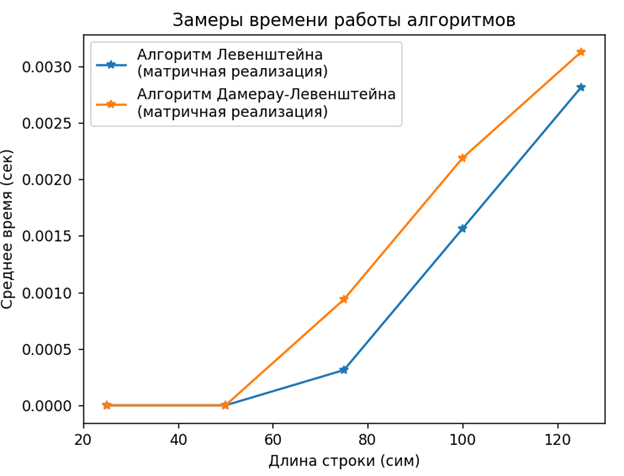
\includegraphics[width=1\textwidth]{graph_mat.png}
    \caption{График времени работы матричных реализаций алгоритмов в зависимости от длин строк}
\end{figure}
\begin{figure}[H]
    \centering
    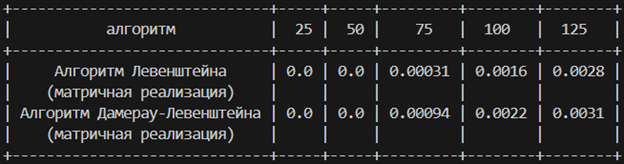
\includegraphics[width=1\textwidth]{table_mat.png}
    \caption{Таблица времени работы матричных реализаций алгоритмов в зависимости от длин строк}
\end{figure}

\begin{figure}[H]
    \centering
    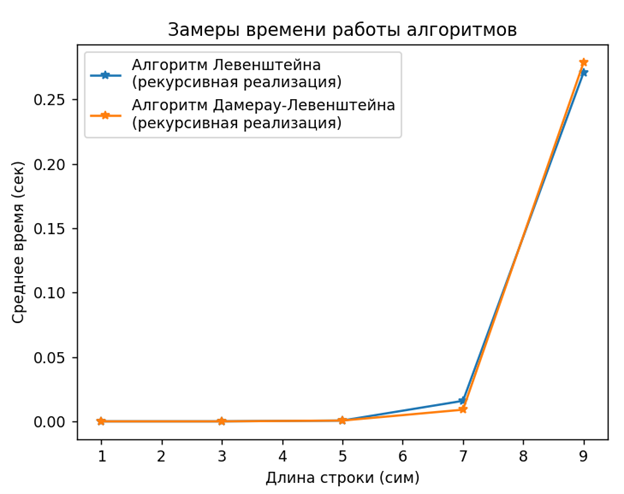
\includegraphics[width=1\textwidth]{graph_rec.png}
    \caption{График времени работы рекурсивных реализаций алгоритмов в зависимости от длин строк}
\end{figure}
\begin{figure}[H]
    \centering
    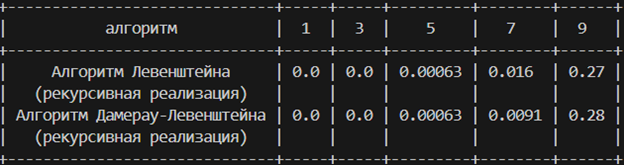
\includegraphics[width=1\textwidth]{table_rec.png}
    \caption{Таблица времени работы рекурсивных реализаций алгоритмов в зависимости от длин строк}
\end{figure}

\begin{figure}[H]
    \centering
    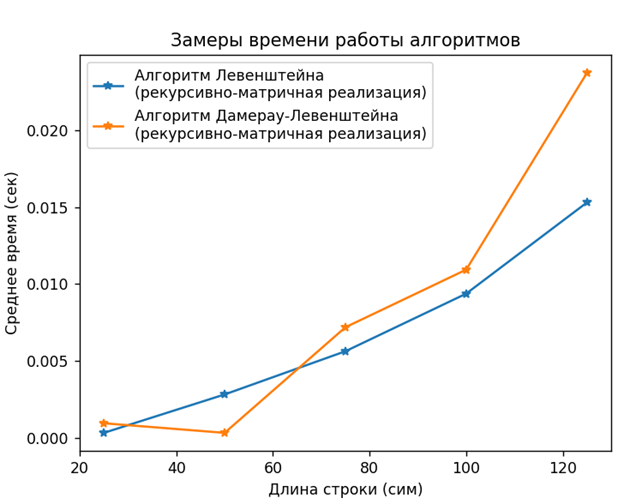
\includegraphics[width=1\textwidth]{graph_rec-mat.png}
    \caption{График времени работы рекурсивно-матричных реализаций алгоритмов в зависимости от длин строк}
\end{figure}
\begin{figure}[H]
    \centering
    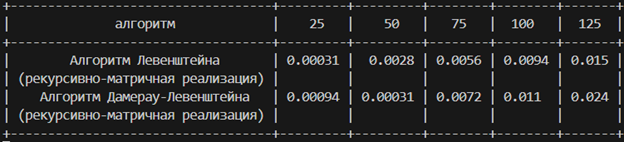
\includegraphics[width=1\textwidth]{table_rec-mat.png}
    \caption{Таблица времени работы рекурсивно-матричных реализаций алгоритмов в зависимости от длин строк}
\end{figure}

Видно, что алгоритм Левенштейна оказался немного быстрее алгоритма Дамерау-Левенштейна из-за дополнительной проверки во втором, что компенсируется меньшей эффективностью первого при наличии перестановок букв в строках.

\subsection{Сравнение работы матричных и рекурсивно-матричных алгоритмов Левенштейна и Дамерау-Левенштейна}
Так как на общем графике матричный и рекурсивно-матричный алгоритмы были очень близки по скорости, были проведены отдельные замеры (на 5-и точках с длиной строк от 25 до 125 символов с шагом 25).
\begin{figure}[H]
    \centering
    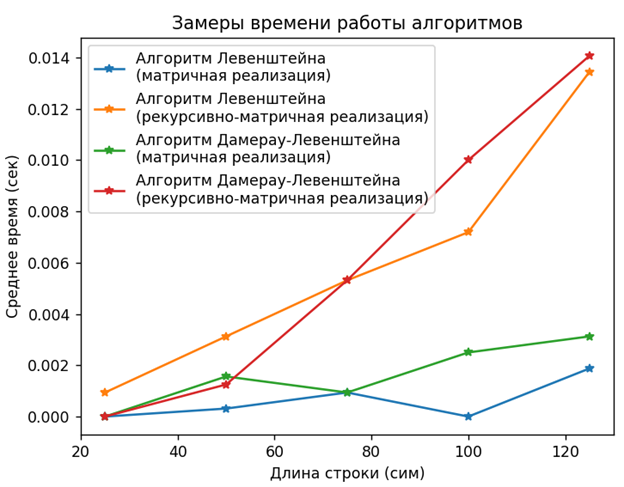
\includegraphics[width=1\textwidth]{graph_mat_rec-mat.png}
    \caption{График времени работы матричных и рекурсивно-матричных реализаций алгоритмов в зависимости от длин строк}
\end{figure}
\begin{figure}[H]
    \centering
    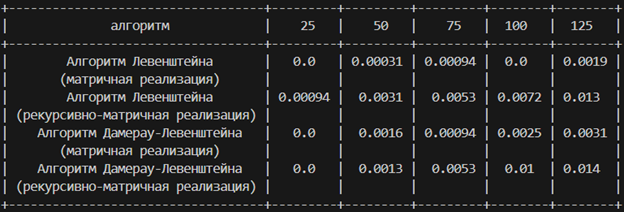
\includegraphics[width=1\textwidth]{table_mat_rec-mat.png}
    \caption{Таблица времени работы матричных и рекурсивно-матричных реализаций алгоритмов в зависимости от длин строк}
\end{figure}

По результатам приведённых графиков видно, что и в алгоритме Левенштейна и Дамерау-Левенштейна рекурсивно-матричный метод работает дольше матричного. Это объясняется затратами на вызов функции при рекурсии и на дополнительные проверки является ли искомое значение уже посчитанным. На небольших длинах строк разница в скорости работы алгоритмов отличается несущественно, однако с увеличением данных растёт и разница во времени.

\subsection*{Вывод}
По результатам проведённых исследований была выявлена большая скорость работы алгоритма Левенштейна над алгоритмом Дамерау-Левенштейна за счёт уменьшения числа проверок, что, однако, даёт иной результат при наличии возможности перестановок символов в строках. При этом матричный вариант выигрывает по скорости в обоих алгоритмах, на втором месте оказался рекурсивно-матричный метод, который делает меньше рекурсивных вызовов, чем рекурсивный метод, и исключает повторные вычисления идентичных веток, так как при вызове каждой новой функции в этом методе передаётся в качестве аргумента ссылка на матрицу, которая хранит уже посчитанные значения, но на эту матрицу также необходима память, а проверки на уже вычисленные значения не всегда приносят положительный результат и занимают время.
\newpage

% Заключение
\section*{Заключение}
В результате выполнения лабораторной работы были исследованы алгоритмы вычисления расстояния Левенштейна и Дамерау-Левенштейна в матричной, рекурсивно-матричной и рекурсивной реализациях.\par
В частности:\par
\begin{itemize}
\item были изучены алгоритмы вычисления расстояния Левенштейна и Дамерау-Левенштейна;
\item применён метод динамического программирования для матричных реализаций алгоритмов;
\item сравнены матричная, рекурсивно-матричная и рекурсивная реализации алгоритмов;
\item сравнены алгоритмы вычисления расстояния Левенштейна и Дамерау-Левенштейна.
\end{itemize}

\newpage


% Список литературы
\begin{thebibliography}{9}
    \bibitem{process_time} Python Documentation. \textit{time.process\_time() - Документация по стандартной библиотеке Python}. Дата обращения: 03 сентября 2024 г. [Электронный ресурс]. Доступно по адресу: \url{https://docs-python.ru/standart-library/modul-time-python/funktsija-process-time-modulja-time/}
    
    \bibitem{tirinox} Tirinox. \textit{Алгоритм Левенштейна на Python: реализация и объяснение}. Дата обращения: 02 сентября 2024 г. [Электронный ресурс]. Доступно по адресу: \url{https://tirinox.ru/levenstein-python/}
    
    \bibitem{gasfild} Гасфилд Дэн. \textit{Строки, деревья и последовательности в алгоритмах}: Информатика и вычислительная биология / Пер. с англ. И. В. Романовского. — СПб.: Невский Диалект; БХВ-Петербург, 2003. — 654 с: ил.
    
    \bibitem{niezov} Ниёзов Д. Л. \textit{Применение методов нечеткого сравнения строк в прикладных задачах}: Выпускная квалификационная работа (Бакалаврская работа). — Тольятти: Тольяттинский государственный университет, 2020. — 45 стр.
    
    \bibitem{levenshtein} Левенштейн В. И. \textit{Двоичные коды с исправлением выпадений, вставок и замещений символов}. Доклады Академий Наук СССР, 1965. 163.4:845-848.
\end{thebibliography}


\end{document}
